%%%%%%%%%%%%%%%%%%%%%%%%%%%%%%%%%%%%%%%%%%%%%%%%%%%%%%%%%%%%%%%%%%%%%%%%%%%%%%%%%%%%%%%%%%%%%%%%%%%
% Chapter 5 -> PHLOWER Experiments and Results
% Author: Mingbo Cheng
%%%%%%%%%%%%%%%%%%%%%%%%%%%%%%%%%%%%%%%%%%%%%%%%%%%%%%%%%%%%%%%%%%%%%%%%%%%%%%%%%%%%%%%%%%%%%%%%%%%
\chapter{PHLOWER Experiments \& Results}
\label{chapter:PHLOWER_bench}

\graphicspath{{chapter5/figs}}

\section{Experiments}
\subsection{Evaluation of trajectory inference}
\subsection{Simulated Data}
\subsection{Execution of trajectory inference}
% List how to install and run the competing methods
% how to set up dynverse environment
\subsubsection{competing methods}
	We first, install dyno(0.1.2) which includes some competing methods of wrapping. To do this, we use devtools::install\_github(``dynverse/dyno'') which includes the dynverse packages dynwrap(1.2.3),  dynmethods(1.0.5.9000), dynplot(1.1.2) and dynfeature(1.0.0). For PHLOWER and STREAM wrapping, we followed tutorial ~\url{https://dynverse.org/developers/creating-ti-method/}. For this, we clone dynclipy(0.1) code from ~\url{https://github.com/dynverse/dynclipy} and use ``pip install .'' to install the package.
\begin{description}
	\item[PHLOWER]
	We need use 
	\item[TSCAN]
	TSCAN has been wrapped in dynmethods, we just pass the ti\_tscan function to dynwrap function infer\_trajectory to infer the trajectory. source code is ~\url{https://github.com/dynverse/ti\_tscan}
	\item[STREAM]
	\item[PAGA] 
	PAGA has been wrapped in dynmethods, we just pass ti\_paga\_tree function to dynwrap function infer\_trajectory to infer the trajectory. source code is ~\url{https://github.com/dynverse/ti\_paga\_tree}
	\item[Monocle3]
	Monocle3 has been wrapped in dynmethods, we just pass the ti\_monocle3 function to dynwrap function infer\_trajectory to infer the trajectory. source code is ~\url{https://github.com/dynverse/ti\_monocle3}
	\item[Slingshot]
	Slingshot has been wrapped in dynwmethods, we just pass ti\_slingshot function to dynwrap function infer\_trajectory to infer the trajectory. source code is ~\url{https://github.com/dynverse/ti\_slingshot}
	\item[Slicer]
	xxx
	\item[slice]
	Slice has been wrapped in dynmethods in ~\url{https://github.com/dynverse/ti\_slice}. However, the simulated data need not log transformation, we adjust ti\_slice code to exclude the transformation part i.e. set ``expression <- exp(expression) - 1'' to be a new wrapper method\_slice. And pass method\_slice function to dynwrap function infer\_trajectory to infer the trajectory.
	\item[RaceID/StemID]
	RaceID/StemID has been wrapped in dynmethods in ~\url{https://github.com/dynverse/ti\_raceid\_stemid}. However, it needs positive input, we adjust ti\_raceid\_stemid code to scale the input data to 0-10 to be a new wrapper method\_raceid\_stemid. And pass method\_raceid\_stemid function to dynwrap function infer\_trajectory to infer the trajectory.
	\item[MST] 
	Minimum spanning tree(MST) is implemented in R package mclust.
	\item[ElPiGraph] 
	ElPigraph has been wrapped in dynmethods, we just pass the ti\_elpigraph function to dynwrap function infer\_trajectory to infer the trajectory. source code is ~\url{https://github.com/dynverse/ti_elpigraph}
	\item[celltree] 
	celltree has been wrapped in dynmethods in ~\url{https://github.com/dynverse/ti\_celltree\_vem}. However, the cellTree source code normalization function ``.normalise.data'' would not work with negative values. We check out cellTree(1.27.0) source code from ~\url{https://git.bioconductor.org/packages/cellTree} and adjust the ``.normalise.data'' function to use 0-1 normalization as the data output for the downstream inference process and recompile cellTree package as the input of dynmethods wrapper. We re-wrap ti\_celltree\_vem code to use the call new cellTree package to be a new wrapper method\_celltree\_vem. And pass method\_celltree\_vem function to dynwrap function infer\_trajectory to infer the trajectory.
	\item[pCreode] 
	pCreode has been wrapped in dynmethods, we just pass the ti\_pcreode function to dynwrap function infer\_trajectory to infer the trajectory. source code is ~\url{https://github.com/dynverse/ti\_pcreode}
\end{description}

\subsection{Evaluation of trajectory inference}
% dynverse benchmarking selected metrics description
The simulated data for trajectory inference. We first described the data source and pre-processing for single cell multi-modal data, next we show how to simulate data for trajectory inference.
\begin{figure}[!ht]
	\centering
	\includegraphics[width=0.95\textwidth]{dynverse_metrics/fig}
	\vspace{0.1cm}
	\caption[dynverse\_metrics]{
	dynverse\_metrics.}
	\label{fig:dynverse_metrics}
\end{figure}

\begin{figure}[!ht]
	\centering
	\includegraphics[width=0.95\textwidth]{evaluation_PHLOWER/fig}
	\vspace{0.1cm}
	\caption[evaluation\_PHLOWER]{
	evaluation\_PHLOWER.}
	\label{fig:evaluation_PHLOWER}
\end{figure}

\section{Results}
\subsection{Apply Trajectory inference to kidney organoid data}
\subsection{Characterize the cell fate xxxx}

\section{Discussion}

